\documentclass[../ImageClassifier.tex]{subfiles}

\begin{document}
    After the prediction an attempt was made to localize the detected class with \ac{grad-cam}, which visualize areas of interest in the last convolutional layer. 
    The idea behind that is the areas where the network was activated must match with the detected object.
    As result we got a heatmap, which matches with the detected object in the image.
    The modified \ac{resnet50} uses images with the width and height of 224 pixels, as result of this the last convolutional layer has 7 x 7 pixel.
    \begin{quoting}[begintext={``}, endtext={''\parencite{grad-cam}}]
      To obtain class-discriminative localization map \(L^c\textsubscript{Grad-CAM} \in \mathbb{R}\textsuperscript{$u \times v$}\) with the width \(u\) and height \(v\) of 7 and \(Z\) is the number of pixels in the feature map, we first compute the gradient of the score for class \(c, y^c\), with respect to feature map activations \(A^k\) of a convolutional layer $\frac{\partial y^c}{\partial A^k}$.
      These gradients flowing back are global averagepooled over the width and height dimensions (indexed by \(i\) and \(j\) respectively) to obtain the neuron importance weights \(a^c_k\):
    \end{quoting}
    \begin{equ}[ht!]
      \begin{equation}
          a^c_k = \overbrace{\frac{1}{Z}\sum \limits_{i}\sum \limits_{j}}^{global\ average\ pooling}\underbrace{\frac{\partial y^c}{\partial A^k_{ij}}}_{gradients\,via\,backprop}
      \end{equation}
      \caption{\parencite{grad-cam}}
      \label{form:grad cam neuron heights}
    \end{equ}
    Now we can calculate the weighted combination of activation maps to follow it by \ac{relu}, because we are only interested in positive influenced pixels for the class of interest.
    Negative pixels belong to other classes in the image \parencite{grad-cam}.
    \begin{equ}[ht!]
      \begin{equation}
          L^c_{Grad-CAM} = \ac{relu} \underbrace{(\sum \limits_{k} a^c_k A^k)}_{linear\,combination}
      \end{equation}
      \caption{\parencite{grad-cam}}
      \label{form:grad cam localization map}
    \end{equ}
    \clearpage
    As result of this calculations we receive a \(7 \times 7\) pixels heatmap with the same size as that of the last convolutional layer in the modified \ac{resnet50}.
    The most important steps are illustrated in figure \ref{fig:grad-cam-process}.
    \begin{figure}[ht!]
      \begin{subfigure}{.24\textwidth}
        \centering
        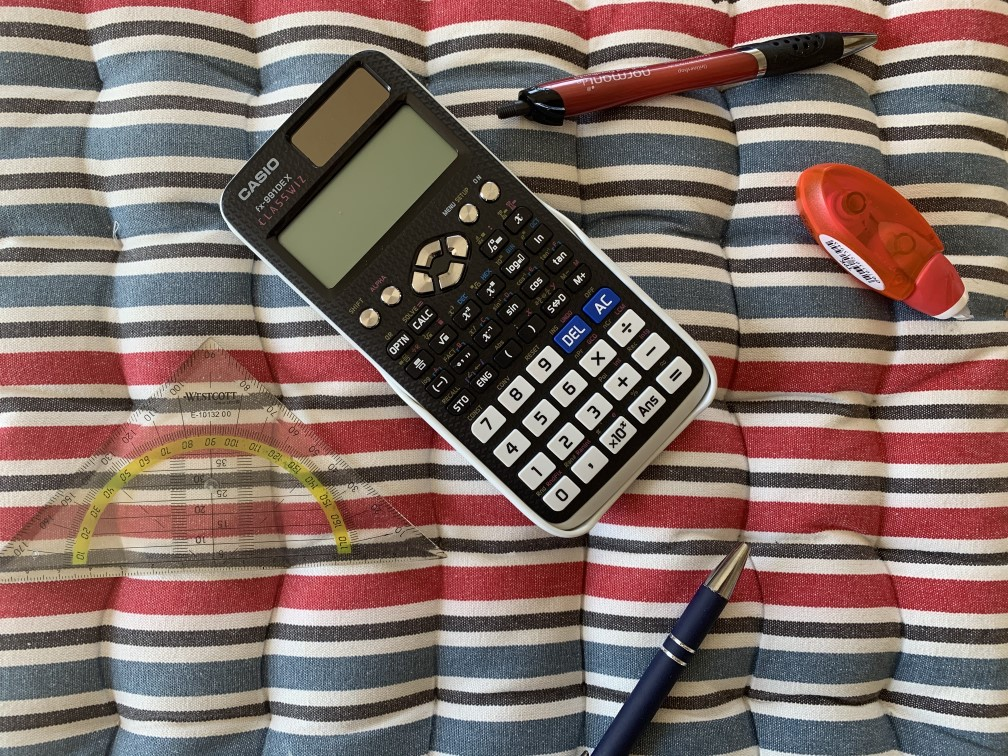
\includegraphics[height=3cm, width=3cm]{./attachments/grad_cam/heatmap_orig.jpg}
        \caption{original image}
        \label{fig:original image}
      \end{subfigure}%
      \begin{subfigure}{.24\textwidth}
        \centering
        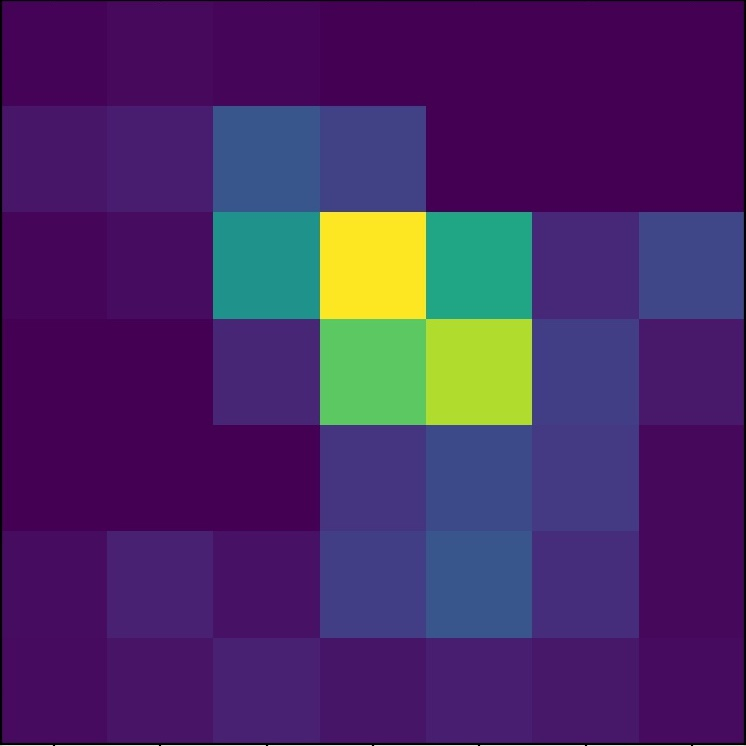
\includegraphics[height=3cm, width=3cm]{./attachments/grad_cam/heatmap.jpg}
        \caption{heatmap activation}
        \label{fig:heatmap activasion}
      \end{subfigure}
      \begin{subfigure}{.24\textwidth}
          \centering
          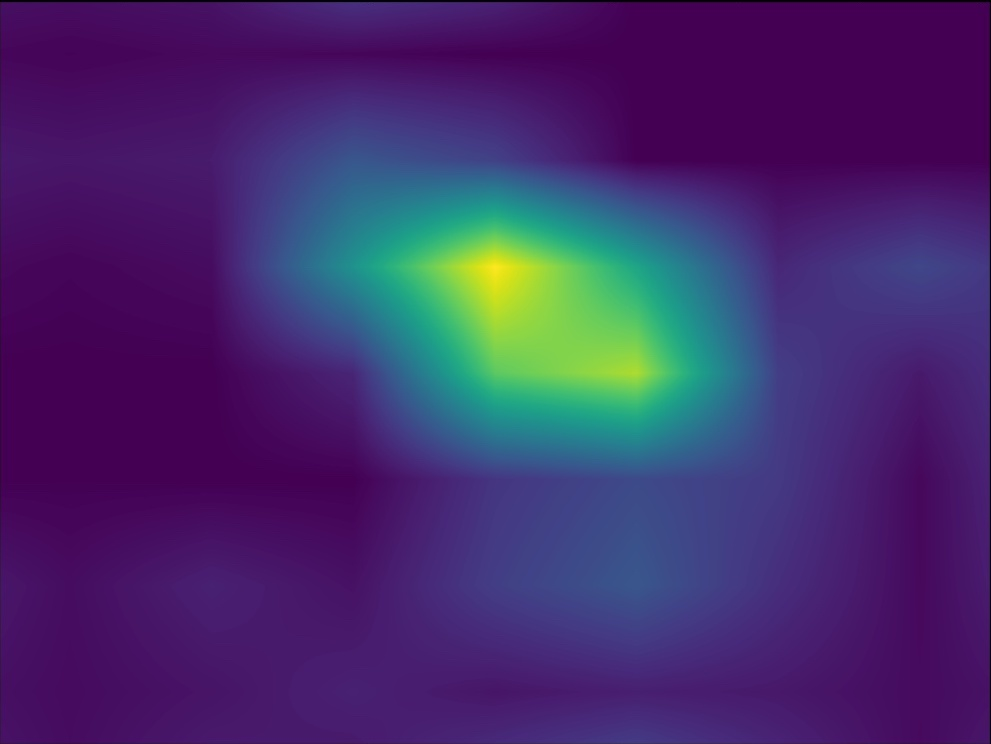
\includegraphics[height=3cm, width=3cm]{./attachments/grad_cam/resized_heatmap.jpg}
          \caption{heatmap resized}
          \label{fig:heatmap resized}
        \end{subfigure}
        \begin{subfigure}{.24\textwidth}
          \centering
          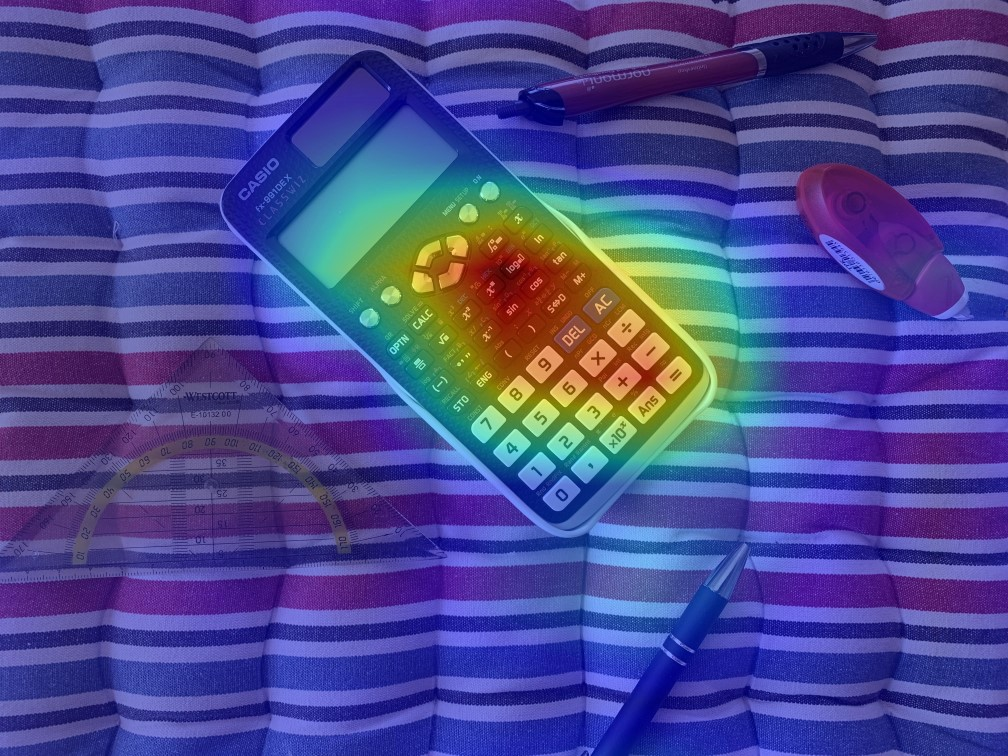
\includegraphics[height=3cm, width=3cm]{./attachments/grad_cam/heatmap_final.jpg}
          \caption{superimposed}
          \label{fig:superimposed image}
        \end{subfigure}
      \caption{Steps of \ac{grad-cam} calculation}
      \label{fig:grad-cam-process}
    \end{figure}

\end{document}
